\documentclass[final,3p,times]{elsarticle}

\usepackage{lipsum}
 \usepackage{graphics}
\usepackage[]{algorithm2e}
 \usepackage{setspace}
%% or use the graphicx package for more complicated commands
 \usepackage{graphicx}
%% or use the epsfig package if you prefer to use the old commands
 \usepackage{epsfig}
 \usepackage{subfigure}

%% The amssymb package provides various useful mathematical symbols
\usepackage{amssymb}
%% The amsthm package provides extended theorem environments
 \usepackage{amsthm,amsmath}
 \usepackage{multirow}
 \usepackage{setspace}
 \usepackage{CJK}
 \usepackage{float}
 \restylefloat{table}
 \onehalfspacing



\makeatletter
\def\ps@pprintTitle{%
	\let\@oddhead\@empty
	\let\@evenhead\@empty
	\def\@oddfoot{}%
	\let\@evenfoot\@oddfoot}
\makeatother


\begin{document}

\begin{frontmatter}

\title{2015 AIMMS-MOPTA competition report, Team RensPolymatheIa}

\author[rvt]{Xin Shen}
\author[rvt]{Jubiao Yang}
\author[rvt]{John E. Mitchell\fnref{fn3}}
\fntext[fn3]{Team Advisor}

\address[rvt]{Rensselaer Polytechnic Institute, Troy, NY 12180}


\end{frontmatter}

\section{Mathematical Formulation for problem without bad luck or with deterministic bad luck}
Our approach to model the system is based upon the observation that the durations of all projects and the time span are integral, therefore the time span can be divided into time segments with equal lengths (one month in this case). A binary variable $X_{jt}$ is assigned to Project $j$ at the $t^{th}$ time segment, which indicates whether Project $j$ starts at the beginning of the $t^{th}$ month. This results in a mixed integer model, which contains the following parameters:

\begin{align*}
	&c_j\,=\, \{\mbox{the cost of Project j}\}\\
	&b_j\,=\, \{\mbox{the benefit of Project j}\}\\
	&d_j\,=\, \{\mbox{the duration of Project j}\}\\
	&c^+_j\,=\, \{\mbox{the added cost to Project j if delayed}\}\\
	&d^+_j\,=\, \{\mbox{the added duration to Project j if delayed}\}\\
	&T \,=\, \{\mbox{the number of months in the total time span, integer}\}
\end{align*}

A binary delay flag $q_j$ is introduced to indicate whether Project $j$ is expected to be delayed, hence the cost and duration of each project under what-if scenarios would be:

\begin{equation}
	\tilde{c}_j = c_j + q_j c^+_j,~~\forall j \in J
\end{equation}

\begin{equation}
	\tilde{d}_j = d_j + q_j d^+_j,~~\forall j \in J
\end{equation}

The following constraints are added to the model:

\begin{itemize}
	
	\item A project can be started at most once throughout the entire time span:
	\begin{equation}
		\label{EqnConstraintStartOnlyOnce}
		\sum\limits_{t=1}^{T} X_{jt}\,\leq\,1,\forall j \in J
	\end{equation}
	
	\item A project cannot be started if it is too late, that is, we can only start a project if it can be finished before the deadline:
	\begin{equation}
		\sum\limits_{t\geq T+1-\tilde{d}_j} X_{jt}\,=\,0, \forall j \in J
	\end{equation}
	
	\item For all $i \nsim j$, i cannot be started within $d_j$ units of time after j started, same for j.
	\begin{equation}
		\sum\limits_{t-\tilde{d}_j+1\leq t'\leq t+\tilde{d}_i-1} X_{jt'}\,+\,X_{it}\,\leq\,1,\forall i \nsim j, \forall t \in \{1 .. T\}
	\end{equation}
	
	\item For all $i \succ j$, j can be started only if i has been finished:
	\begin{equation}
		\label{EqnPrecedence}
		\sum\limits_{t'\leq t-\tilde{d}_i} X_{it'} \,\geq\, X_{jt},\forall i\succ j, \forall t \in \{1 .. T\} 
	\end{equation}
	
	\item For all $I\,\vdash\,j$, j cannot be started until at least one of the projects in I has been finished:
	\begin{equation}
		\label{EqnAnyPrecedence}
		\sum\limits_{i\in I}\sum\limits_{t'\leq t-\tilde{d}_i} X_{it'}\,\geq\,X_{jt},\forall I\,\vdash\,j, \forall t \in \{1 .. T\}
	\end{equation}
\end{itemize}

Apparently Constraint (\ref{EqnPrecedence}) is a special case of Constraint (\ref{EqnAnyPrecedence}), with only Project $i$ rather than multiple elements in Set $I$, and can thus be generalized into Constraint (\ref{EqnAnyPrecedence}) for simplicity.

The objective function is defined as:

\begin{equation}
	NPV_{\gamma} ( S,T ) = - \sum\limits_{\substack{j \in S\\0 \leq t_j/12 \leq 3}} \gamma^{t_j} \tilde{c}_j + \sum\limits_{\substack{j \in S\\0 \leq (t_j+\tilde{d}_j)/12 \leq 3}} \gamma^{t_j+\tilde{d}_j} \tilde{b}_j
\end{equation}

In the optimization problem, it is written as:
\begin{equation}
	NPV_{\gamma} ( S,T ) = - \sum\limits_{i,t} \gamma^t \cdot \tilde{c}_i \cdot X(i,t) + \sum\limits_{i,t} \gamma^{t+\tilde{d}_i} \cdot \tilde{b}_i \cdot X(i,t)
\end{equation}

It is easy to construct the one-to-one correspondence between (S, T) and X, where:
\begin{equation}
	S\,=\,\{i | \exists t,~\mbox{s.t.}~X(i,t)=1\}\;
\end{equation}
and for each element $t_i$ in T, which is the starting time of project i in S:
\begin{equation}
	t_i~=~t ,~~~\mbox{where}~ X(i,t)=1
\end{equation}

Thus to get the optimal schedule without bad luck or with deterministic bad luck, we can formulate the optimization problem as:
\begin{equation}
	\begin{array}{ll}
		\max\limits_{X} &NPV_\gamma(S,T)\\
		s.t &(\ref{EqnConstraintStartOnlyOnce}) -(\ref{EqnAnyPrecedence})\\
		& X_{it} \in \{0,\,1\}
	\end{array}
\end{equation}

The above model can be efficiently solved by typical MIP solvers such as Cplex.

\section{Scheduling Under Bad Luck}
From now on, the problem is to take failures and delays into consideration while determining the project portfolio. A parameter $W\geq 0$ is introduced to represent the budget of bad luck. We define:
\begin{align*}
	&I_f\,=\, \{\mbox{Project that will be failed by the bad luck}\}\\
	&I_{\delta}\,=\, \{\mbox{Project that will be delayed by the bad luck but eventually will succeed}\}\\
	&I_{f|\delta}\,=\, \{\mbox{Project that will be delayed by the bad luck and eventually will fail}\}\\
\end{align*}

Each project has probabilities to delay, to fail, or to delay and then fail. The probabilities can help with calculation of information entropy, which is used to measure the cost of each occurrence of bad luck. The total cost of bad luck is defined as:
\begin{equation*}
	w(I_f, I_{\delta}, I_{f|\delta})\,:=\,\sum_{j\in I_f} [-log_2(p_{f,j})]\,+\,\sum_{j\in I_{\delta}}[-log_2((1-p_{f,j})p_{\delta,j})]\,+\,\sum_{j\in I_{f|\delta}}[-log_2((1-p_{f,j}))]
\end{equation*}

Our purpose is to find a schedule that yields the highest profit under certain budget of bad luck. A general formulation is the following maxmin problem:
\begin{equation}\label{SecondOrProblem}
	\begin{aligned}
		\max_{S,T}&\qquad\min_{I_f, I_{\delta}, I_{f|\delta}}\qquad NPV_{\gamma}'(S,T,I_f, I_{\delta}, I_{f|\delta})\\
		subject to \qquad & i\,\succ\,j,\,\forall (i,j)\,\in\,E,\\
		& i \,\neq \,j, \,\forall (i,j)\,\in\,E',\\
		& I \,\vdash \,j, \,\forall (I,j)\,\in\,E'',\\
	\end{aligned}
\end{equation}

The net present value of the portfolio is computed by summing up the costs and benefits of all projects in the schedule, discounted appropriately at the time they are incurred:
\begin{equation}
	NPV_{\gamma}(S,T)\,=\,\sum_{j\in S, 0\leq t_j/12<3} \gamma^{t_j} \tilde{c}_j\,+\,\sum_{j\in S, 0\leq t_j/12<3} \gamma^{t_j+d_j} \tilde{b}_j
\end{equation}

\section{Adaptive Scheduling of Projects}

In practice, the original schedule is subject to update once any bad luck occurs. For example, consider a scenario where an intermediate project delays, which could lead to inability of some other projects to be completed in time. Although we can continue with the subsequent projects, a possible better option could be to remove a proportion of projects while updating the schedule. The purpose is to reduce the potential loss based upon information at the current stage. Our analysis will take the update into consideration. At each time $t^{badluck}$ when a bad luck happens, the update must follow the rules:
\begin{itemize}
	\item Only projects selected in the original schedule can be chosen in the updated schedule.
	\item The update will take place when a bad luck occurs, and we assume that bad luck only occurs at the scheduled ending time of a project. The cases where projects delay and then fail can be regarded as special occasions where bad luck occurs twice, in which the first time is at the scheduled ending time of the previous plan, when we know the project is delayed, and the second time is the moment it fails at the end of the delay.
	\item Only the projects that are scheduled at and after the current bad luck can be rescheduled.
	\item The bad luck that has not happened is unknown. When updating the schedule, we make an optimal choice without assuming that bad luck will take place after $t^{badluck}$. 
\end{itemize}



With the assumptions above, the realized schedule can be obtained by solving a series of optimization problems.We begin with an initial schedule $(S,T)$, which can be the solution in part 1, and at each time $t_i$ when bad luck occurs to a single project, the schedule is updated to $(S_i, T_i)$ based upon current progress and the type of bad luck at $t$. Let $(S_{i-1},T_{i-1})$ be the schedule after last bad luck happens at time $t_{i-1}$ with corresponding decision variable $X'_{i,t}$, and $(I_{tf}, I_{t\delta})$ be the set of projects that has delayed or failed before and at time t. If at time t we know a project has been delayed and failed, we put the project into both set $I_{tf}$ and $I_{t\delta}$. Otherwise, if we only get the information that the project has been delayed, the project will only be selected into the set $I_{tf}$. We can find an updated schedule$(S_{i},T_{i})$ after bad luck at time $t$ by solving a problem which has the following constraints with decision variable $X_{i,t}$:
\begin{itemize}\label{StartCon1}
	\item As in part 1, a single project can only be started at most once.
	\begin{equation}
		\sum\limits_{t} X_{it}\,\leq\,1,\forall i
	\end{equation}
	\item As with part 1, the starting time of a project cannot be too late. To evaluate the effect of delay, since we have already assumed that no bad luck will happen after time t,it's worth to note that no delay except for the projects in set $I_{t\delta}$ will be considered while determining the updated schedule.
	\begin{equation}
		\label{EqnStartOnlyOnce2}
		\sum\limits_{t\geq T+1-d_i} X_{it}\,=\,0, \forall i
	\end{equation}
	\item The realized schedule, i.e, the schedule prior to time $t$ cannot be changed:
	\begin{equation}
		X_{i,t}\,=\,X'_{i,t}, \forall t < t_i
	\end{equation}
	%\begin{itemize}
	\item For any $i\succ j$, if $i\notin I_{tf}\cup I_{t\delta}$, j cannot be started until i has been finished.                 
	\begin{equation}
		\sum\limits_{t'\leq t-d_i} X_{it} \,\geq\, X_{jt'},\forall t 
	\end{equation} 
	\item For any $i\succ j$, if $i\in I_{tf}$, j cannot be started at any time.
	\begin{equation}
		\sum\limits_{t} X_{jt}\,=\,0
	\end{equation}
	\item For any $i\succ j$, if $i\in I_{t\delta}$,j cannot be started until i hazs finished.
	\begin{equation}
		\sum\limits_{t'\leq t-d_i-d^+_i} X_{it} \,\geq\, X_{jt'},\forall  t 
	\end{equation}
	\item For all $i \nsim j$, i cannot be started within $d_j$ units of time after j started. The same applies for j.
	\begin{equation}
		\sum\limits_{t-\tilde{d}_j+1\leq t'\leq t+\tilde{d}_i-1} X_{jt'}\,+\,X_{it}\,\leq\,1, \forall t 
	\end{equation}
	\item For any $I \vdash j$, j can be started only if at least one project in set $I$ has been successfully finished. 
	\begin{equation}
		\sum\limits_{p \in (I/\{ I_{tf})\cap I_{t\delta}}\sum\limits_{t'\leq t-d_p-d^+_p} X_{pt'}+\sum\limits_{p \in (I/\{ I_{tf})\cap \bar{I_{t\delta}}}\sum\limits_{t'\leq t-d_p} X_{pt'}\,\geq\,X_{jt}, \forall t
	\end{equation}
	\item Projects that are not selected in the initial schedule $(S,T)$ will not appear in the updated schedule
	\begin{equation}\label{EndCon}
		X_{it}\,=\,0, \forall i \notin S_0 
	\end{equation}
	%\end{itemize}
	%\item For any project i which is delayed at time t,
	%\begin{itemize}
	
	%\end{itemize}
\end{itemize}
Thus given the schedule $(S_{i-1},T_{i-1})$, the updated schedule $(S_i, T_i)$ after bad luck happens at time $t_i$ can be acquired by solving the optimization problem:
\begin{equation}\label{UpdateOpt}
	\begin{array}{ll}
		\max\limits_{X} &NPV(S_i,T_i)\\
		s.t &(\ref{EqnStartOnlyOnce2}) -(\ref{EndCon})\\
		& X_{it} \in \{0,\,1\}
	\end{array}
\end{equation}
The algorithm to get the final realization of the original schedule with the given triple of bad luck $(I_f, I_{\delta}, I_{f|\delta})$ is as follows:\\
\begin{algorithm}[H]
	\KwData{Initial Schedule $(S_0,T_0)$, Triple of bad luck $(I_f, I_{\delta}, I_{f|\delta})$}
	\KwResult{Final Realization (S',T')}
	(S1,T1)\,=\,(S,T)\;
	\While {$(I_f, I_{\delta}, I_{f|\delta})$ is not empty}{
		Choose a bad luck in $(I_f, I_{\delta}, I_{f|\delta})$ with the earliest time of occurrence\;
		Update the set $(I_{tf}, I_{t\delta})$, which is the set of bad luck that we know has happened\;
		%Remove i from $(I_f, I_{\delta}, I_{f|\delta})$\;
		Solve the problem (\ref{UpdateOpt})\;
		Remove 
	}
	Output $(S',T')=(S_n,T_n)$, where n is the last time bad luck occurs.
\end{algorithm}

\section{Estimation of Worst Case Scenario}
In the previous section we developed an algorithm to update the schedule when any bad luck occurs. Given an initial schedule $(S, T)$, we can get a final realization $(S', T')$ after all the bad luck in the triple $(I_f, I_{\delta}, I_{f|\delta})$  take s place.  The impact of bad luck can be quantified by the loss it incurs. The loss is calculated as the difference between the NPV value of the initial schedule and the realized schedule, which can be expressed as:
\begin{equation}
	Loss_{(S,T)}(S',T')\,=\, NPV(S',T')\,-\,NPV(S,T)
\end{equation}
The question arises that given a budget of bad luck, which selection of the triple $(I_f, I_{\delta}, I_{f|\delta})$  will lead to the maximum loss. A brute force approach for assessing the worst selection of the triple is to try every combination of bad luck and choose the one with the largest loss. However, because of our limited source of computing and the size of the problem, the method is computationally infeasible especially when the number of projects grows extremely large, since there will be exponential number of choices of the triple. 

An alternative method is the greedy heuristic, which  aims at finding a triple $(I_f, I_{\delta}, I_{f|\delta})$ with a large loss and is also computationally tractable. We begin with an empty triple  $(I_f, I_{\delta}, I_{f|\delta})$ and iterate based upon the current budget of bad luck and bad luck remained. In every iteration, we add a project with certain type of bad luck that yields the most loss to the triple and update the realization of the schedule. The iteration terminates when no bad luck that incurs loss can be added to the triple. The algorithm provides a way to get a bad realization of schedule and helps identify the key components in the schedule, although there's no theoretical proof for the worst. The algorithm is:
\linebreak
\begin{algorithm}[H]\label{EstimateWorst}
	\KwData{Initial Schedule (S,T), budget of bad luck W}
	\KwResult{Triple of bad luck in the worst case $(I_f, I_{\delta}, I_{f|\delta})$}
	\While{1}{
		\For{i in S, p in $\{Failure, delay, delay and failure\}$ with $W_{ip}\leq W$}{
			Find the updated schedule (S',T') by solving the optimization problem if with the triple of bad luck contains previously selected bad luck and type p bad luck assigned to project i\;
			Compute the loss, which is the total benefit of the plan subject only to the previouly selected bad luck minus the result in the last step\;
		}
		\eIf{There exist some project i with type bad luck that incurs positive loss}{
			pick the one that with the most loss, or the highest ratio of loss over $W_{ip}$\;
			W=W-$W_{ip}$\; 
		}{
		Jump out of the loop\;
	}
}
\end{algorithm} 


\section{Robustification of Schedule}
In the last section we apply the greedy heuristic in the last section to identify projects in the worst case scenario, which can be regarded as vulnerable to bad luck and plays an important role in the scheduling network. Given the set of these weak but important components in the schedule, we take several strategies to for robustification based upon the type of bad luck, including:
\begin{itemize}
	\item If project i fails in the worst case scenario:
	\begin{itemize}
		\item i is the single project chosen in set I with $I\vdash j$ and j is also in the original schedule. Add another project $k\in I$ to the schedule. 
		\item Delete project i. This might result in:
		\begin{itemize}
			\item i and subsequent projects which depend on i will not start
			\item other projects which have conflict with i but not selected will start.
		\end{itemize}
	\end{itemize}
	\item If project i is delayed in the worst case scenario:
	\begin{itemize}
		\item Move the starting time of i forward if possible.
		\item Delete the project i. This may cause the same consequence as with the case of failure.
	\end{itemize}
	\item if project i is delayed and then failed in the worst case scenario. The treatment can be a combination of that in the case of delay and case of failure.
\end{itemize}
There are also many other strategies which are not covered in our program, for example, under the condition of adaptive scheduling, the starting time of certain projects, which are prerequisite to many other projects but also highly susceptible to failure, can be moved forward. If they fail, other projects won't start.\\

Note that the above strategies does not necessarily yield a solution whose worst scenario is better than before. So each time we made a single or a set of changes to the original plan, we need to check whether the worst case of updated one is better than the previous one.


\section{Computational Results}
\subsection{Smaller Dataset}
In the second problem, we begin with the solution, where we assumed that no bad luck happens. The greedy heuristic (\ref{EstimateWorst}) can be applied here. For purpose of illustration we calculate the loss for every possible bad luck happened to a single luck no matter whether the bad luck required is more than the budget. Table \ref{TableLossIncurGammap99} gives the loss that incurred by each single occurrence of bad luck when the constant $\gamma$ is equal to 0.99.

\begin{table}[H]
	\centering
	\begin{tabular}{|c|c|c|c|}
		\hline
		project & Failure & Delay and Failure & Delay \\
		\hline
		Job1 & -12.2333 & -12.3193 & -12.3193 \\
		\hline
		Job2 & -12.2333 & -12.3193 & -12.3193 \\
		\hline
		Job4 & -12.2333 & -12.3135 & -12.3135 \\
		\hline
		Job6 & -12.2333 & -12.3211 & -0.08775 \\
		\hline
		Job8 & -6.11092 & -6.30892 & -0.198 \\
		\hline
		Job9 & -7.77821 & -7.95372 & -0.1755 \\
		\hline
		Job10 & -13.789 & -13.9445 & -0.15556 \\
		\hline
	\end{tabular}
	\caption{Loss incurred by each single bad luck occurrence, $\gamma=0.99$}
	\label{TableLossIncurGammap99}
\end{table}

We study several combinations of $\gamma$ and $W$. 
\begin{itemize}
	\item We begin with a simple case $W=1$ and $\gamma=0.99$. It is obvious that none of the bad luck will happen, which is shown in Figure \ref{FigData1hp990w1p000}.
	
		\begin{figure}[H]
			\centering
			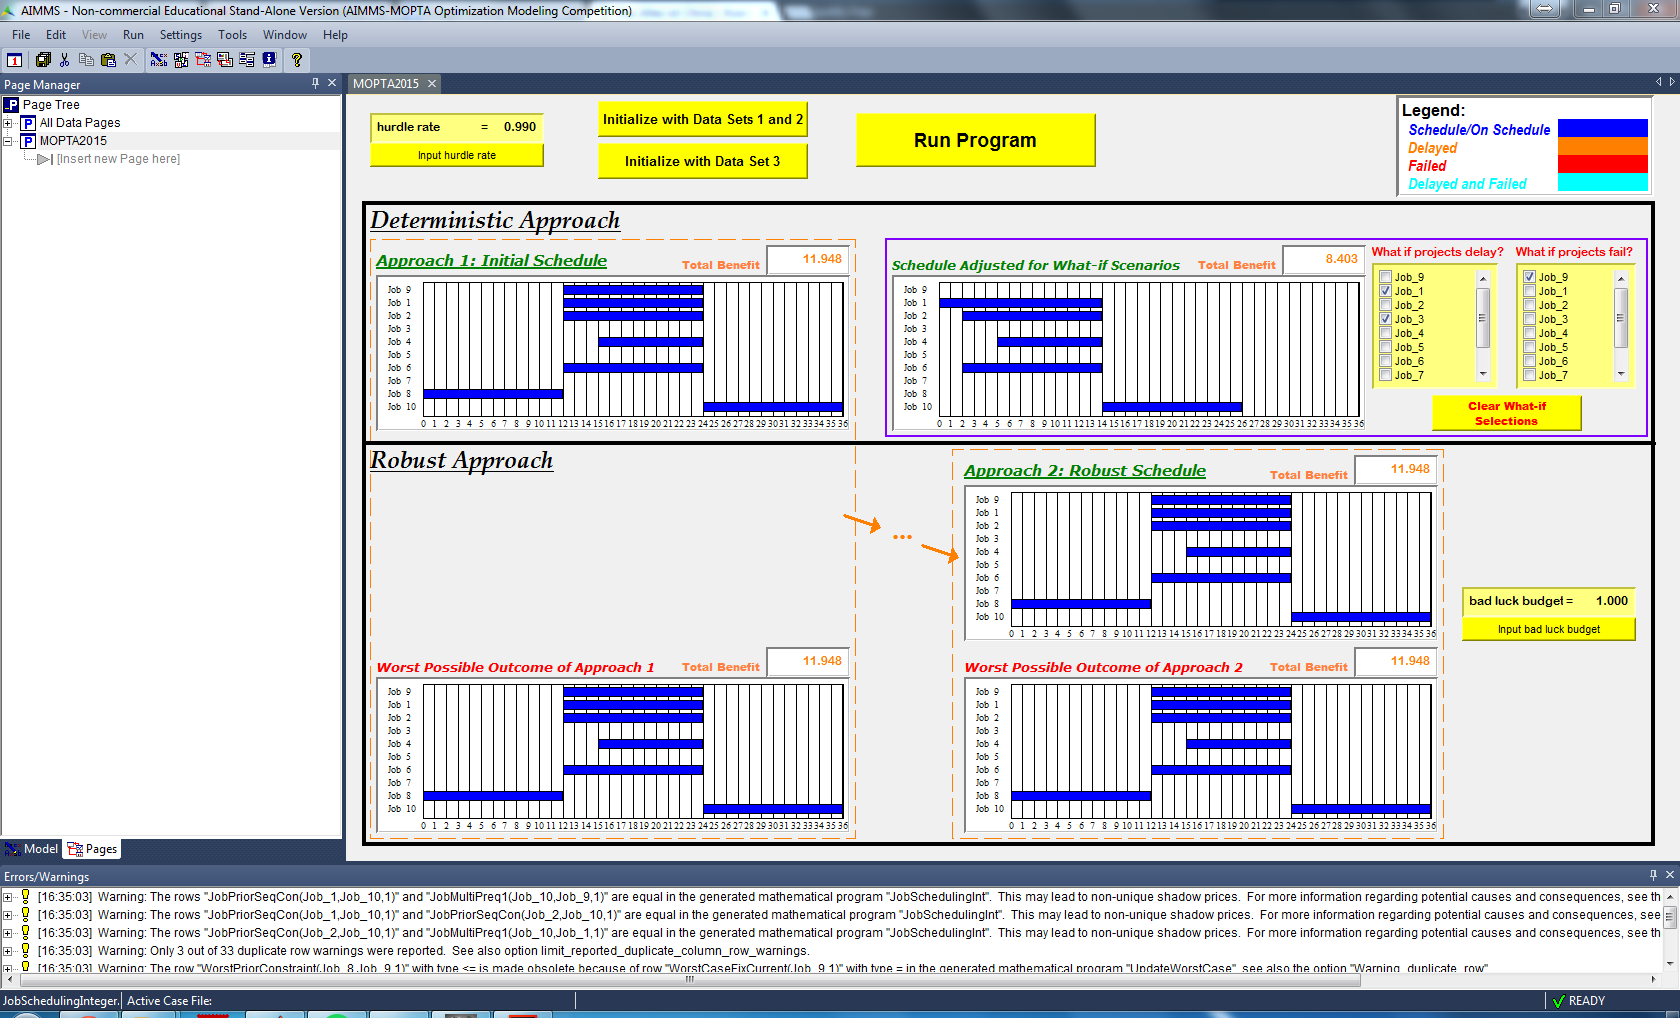
\includegraphics[trim=110mm 40mm 5mm 25mm, clip, width=14cm]{Data1hp990w1p000.png}
			\caption{GUI with result, $W=1.0$, $\gamma=0.99$}
			\label{FigData1hp990w1p000}
		\end{figure}
	
	\item When the budget $W=1.4$ and $\gamma=0.99$. The above table gives the loss of each potential choice of bad luck. When $W$ equals $1.4$ it reaches the threshold for Project 4 to fail. In the worst case scenario, Project 4 fails and Project 1 cannot be started. Two alternatives are considered. In the first approach, all decision variable for Project 4 are fixed to be 0, while in the second approach, we'll add Project 3 since $\{3,4,5\}\vdash 10$, as the failure of Project 4 leads to failure of Project 1. The worst case scenario of the results of the two alternatives are examined, and worst case in the result of second approach is better than both the previous result and Approach 1. Therefore we add 3 into the plan and update the chart of loss to Table \ref{TableLossIncur} listed below.

		\begin{table}[H]
			\centering
			\begin{tabular}{|c|c|c|c|}
				\hline
				project & Failure & Delay and Failure & Delay \\
				\hline
				Job1 & -12.2333 & -12.3193 & -12.3193 \\
				\hline
				Job2 & -12.2333 & -12.3193 & -12.3193 \\
				\hline
				Job4 & -3.55E-15 & -0.08016 & -0.08016 \\
				\hline
				Job6 & -12.2333 & -12.3211 & -0.08775 \\
				\hline
				Job8 & -6.11092 & -6.30892 & -0.198 \\
				\hline
				Job9 & -7.77821 & -7.95372 & -0.1755 \\
				\hline
				Job10 & -13.789 & -13.9445 & -0.15556 \\
				\hline
				Job3 & -12.2333 & -6.39589 & -6.39589 \\
				\hline
			\end{tabular}
			\caption{Loss incurred by each single bad luck occurrence, $\gamma=0.99$}
			\label{TableLossIncur}
		\end{table}
		
		The final schedule is highly resilient to bad luck at the level of $W$, as is shown in Figure \ref{FigData1hp990w1p400}.
		
		\begin{figure}[H]
			\centering
			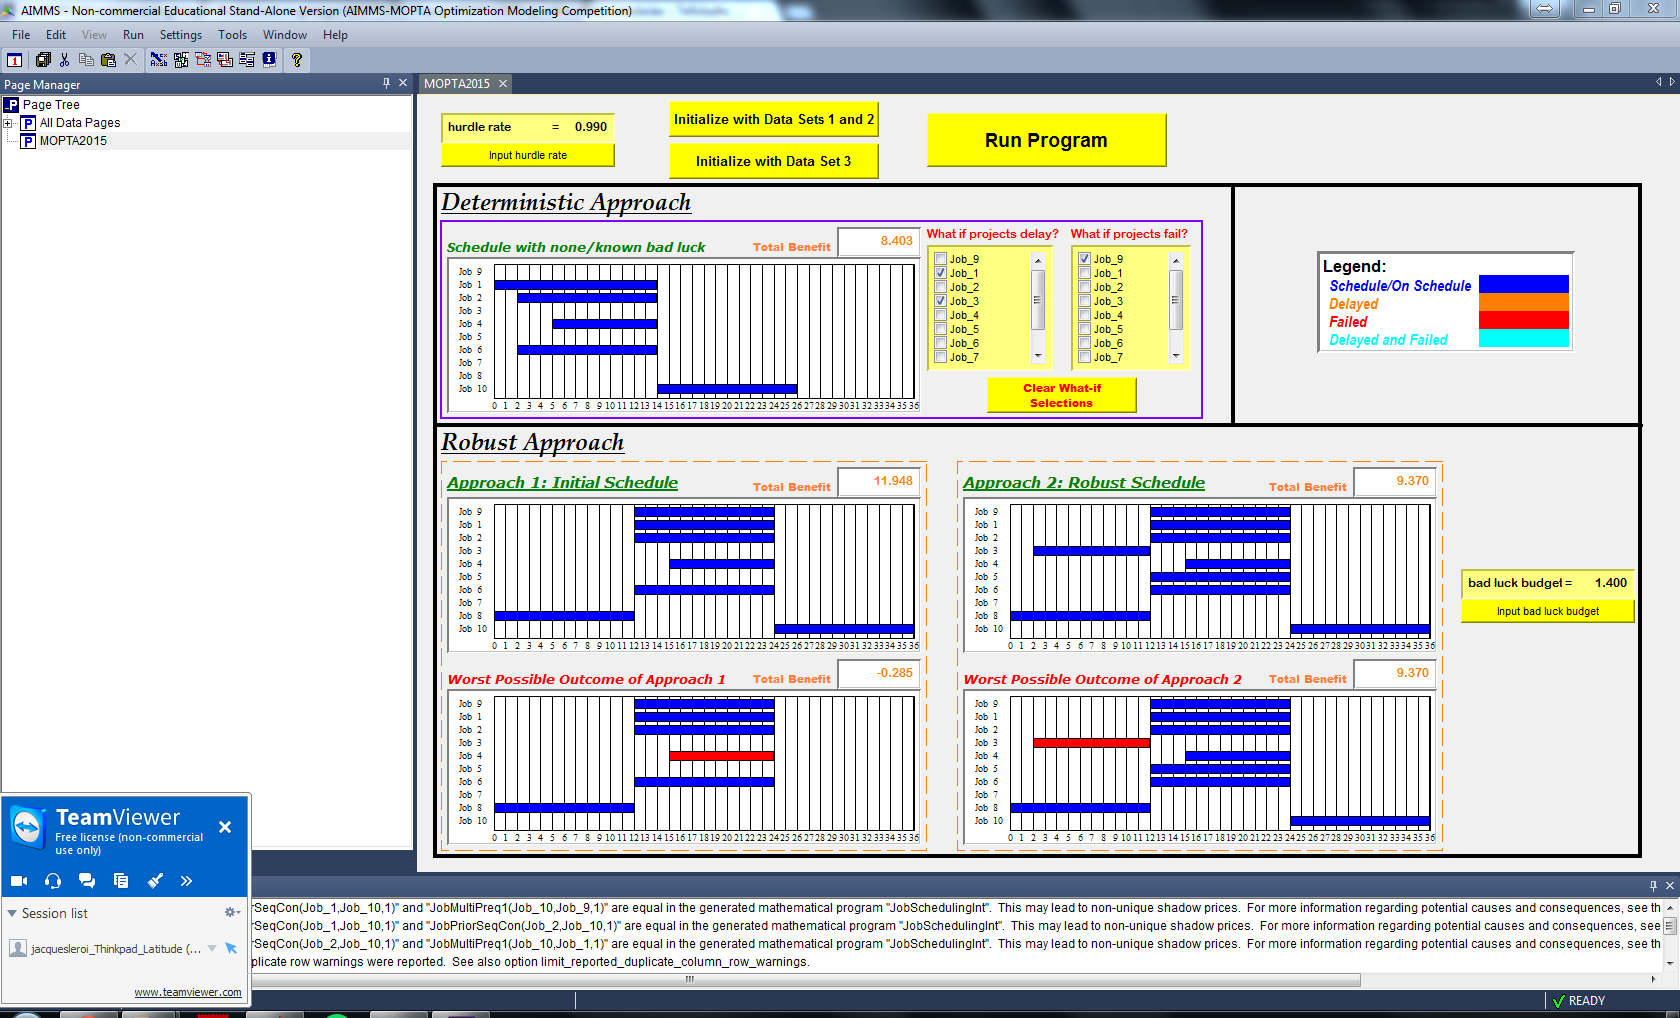
\includegraphics[trim=110mm 40mm 5mm 25mm, clip, width=14cm]{Data1hp990w1p400.png}
			\caption{GUI with result, $W=1.4$, $\gamma=0.99$}
			\label{FigData1hp990w1p400}
		\end{figure}

	\item When the budget $W=2.5$ and $\gamma=0.99$. Under this condition the failure of Project 1 will lead to the most loss. The only possible method for improvement is to restrict decision variable corresponding to Project 1 to be 0. In the resulting scheduling net work we only have the Project 8 and Project 9.
	
		\begin{figure}[H]
			\centering
			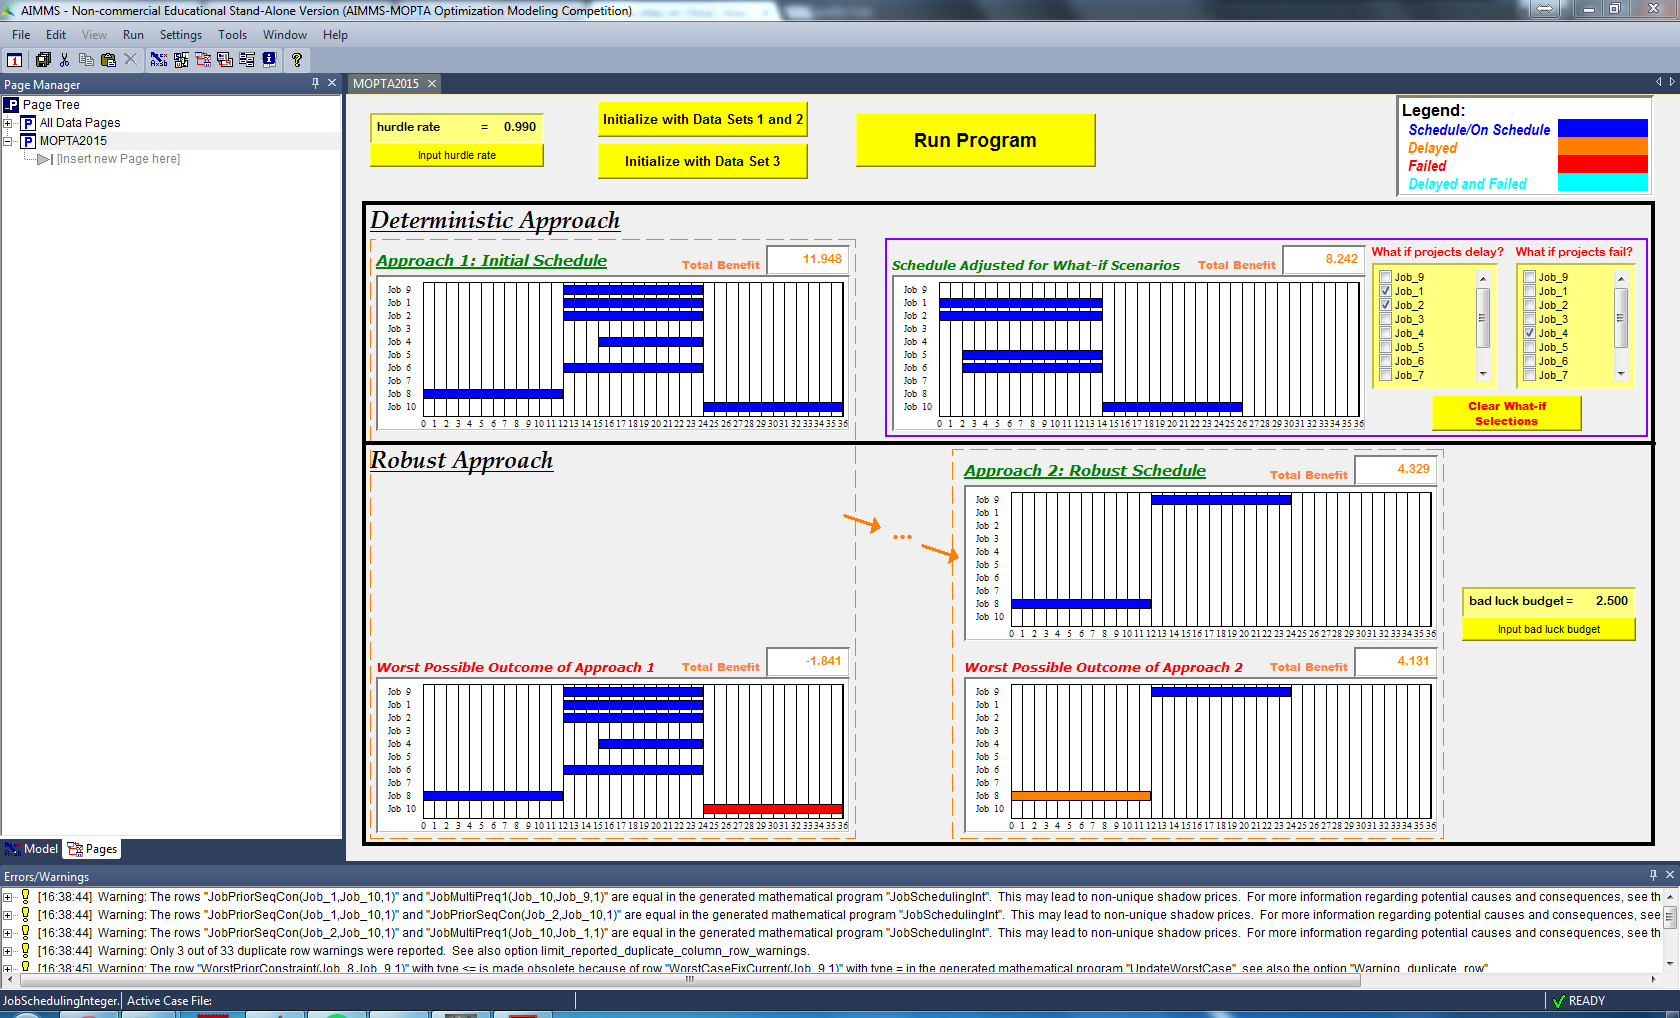
\includegraphics[trim=110mm 40mm 5mm 25mm, clip, width=14cm]{Data1hp990w2p500.png}
			\caption{GUI with result, $W=2.5$, $\gamma=0.99$}
			\label{FigData1hp990w2p500}
		\end{figure}
		
		As $W$ goes larger both Projects 9 and 10 would fail and the best choice would be doing nothing.

	\item When the budget $W=2.5$ and $\gamma=0.95$,  we can observe a dramatic change in the intial condition from the case $\gamma=0.99$. Only Project 8 and Project 9 are selected in the initial schedule. The schedule is highly vulnerable to delay, since the bad luck that will result in the most loss is delay for Project 8. Since Project 8 cannot be moved forward, the only way that may lead to a better solution is to delete Project 8. The resulting schedule contains no projects and of course will no longer be influenced by bad luck.
	
		\begin{figure}[H]
			\centering
			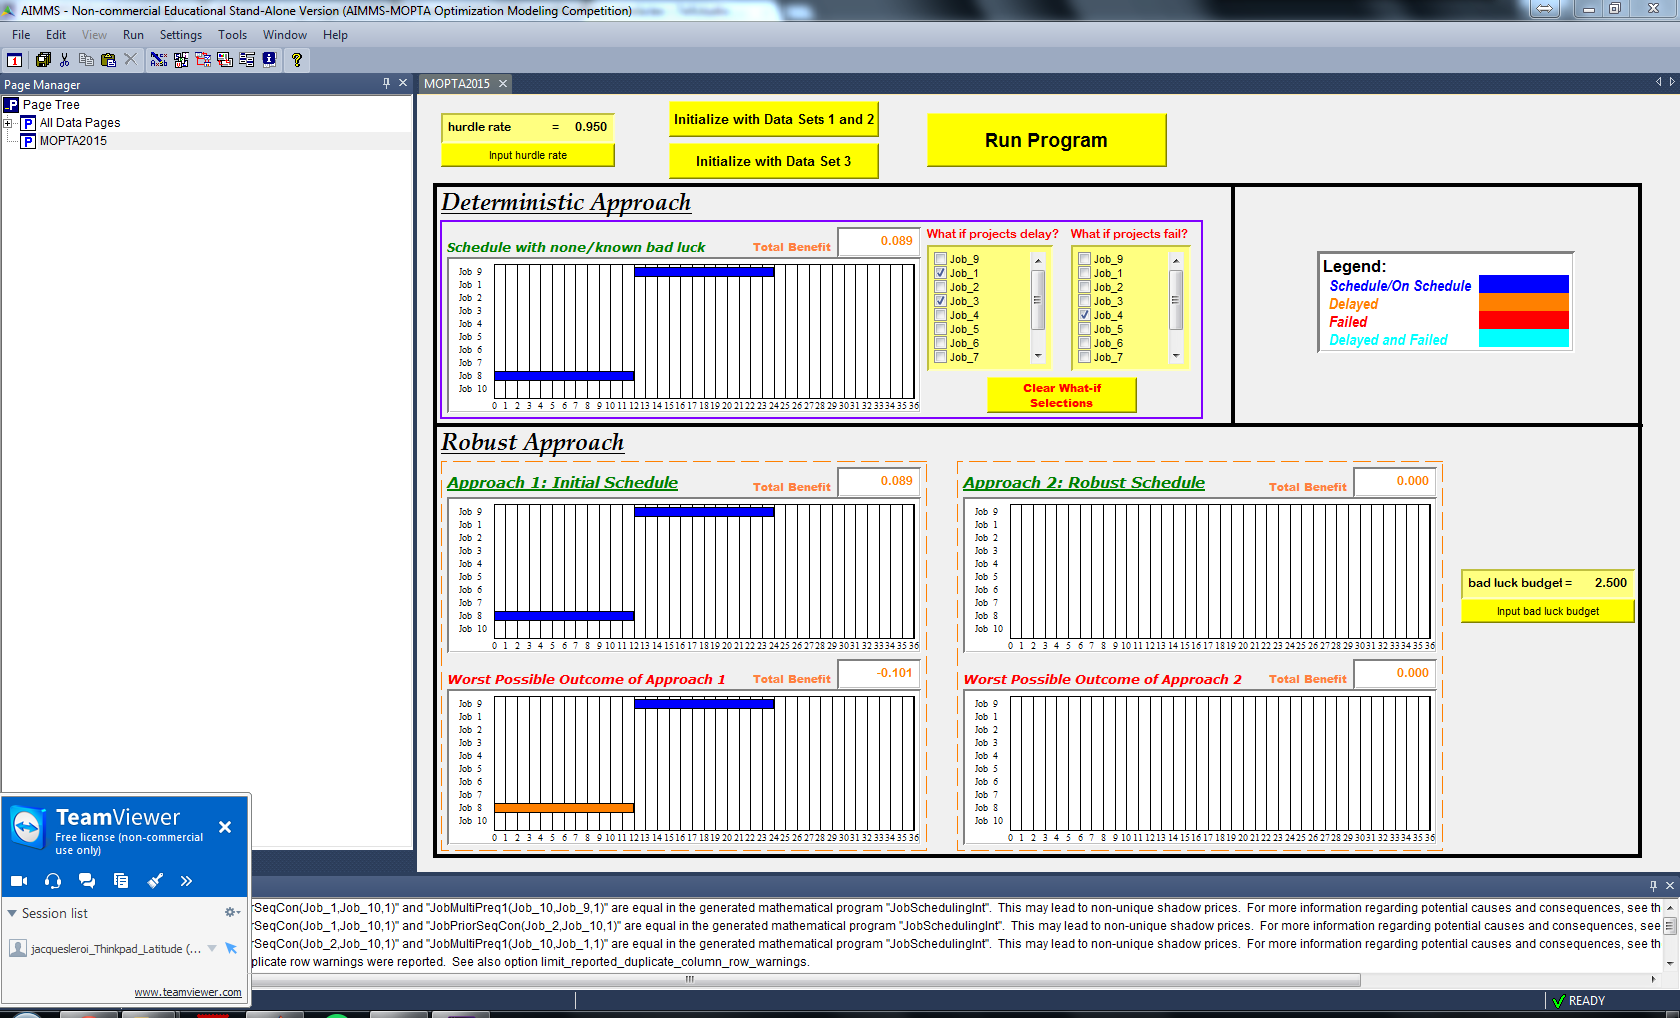
\includegraphics[trim=110mm 40mm 5mm 25mm, clip, width=14cm]{Data1hp950w2p500.png}
			\caption{GUI with result, $W=2.5$, $\gamma=0.95$}
			\label{FigData1hp950w2p500}
		\end{figure}
\end{itemize}
 
\subsection{Larger Dataset}
Similar to the case of the smaller dataset, for the large data set our analysis will begin with the result with Approach 1, which does not take any risk of failure or delay into consideration. Greedy algorithm still plays a central role in acquiring the worst case scenario. However, in the case of the larger dataset, which contains 76 projects, it is time consuming to perform analysis on the loss incurred by every single occurrence of bad luck since the formulated optimization problem has thousands of variables. Two strategies are taken based upon the observation of the initial result from Approach 1:
\begin{itemize}
\item Most projects starts before the 18th month, which implies that even delay takes place, it is unlikely that there will be any project that cannot be completed in time. And currently we only limit our discussion to the case where the hurdle rate is large,i.e, greater than $0.99$, thus the discount effect, together with additional cost of delay is trivial and the resulting loss of delay is rather negligible when compared with that of failure. Another observation is that in many projects, the budget of failure is comparable to that of delay. As a result, in our analysis for the large data set we'll assume that bad luck only happens in the form of failure.
\item Instead of giving a precise estimation of the loss of each occurrence of bad luck, we adopted the following algorithm to find a naive estimation of the failure of a single project.

\begin{algorithm}
\KwData{Current  Realization of Schedule (S',T')}
\KwResult{Loss(S,'failure'), each entry represents the naive estimate of loss incured by only failing the corresponding entry in S under current realization}
$S''\,=\,\{\}$\;
\While{S' is not empty}{
    Pick $i\in S'$ with the latest starting time.\;
    Loss(i)=$b_i*\gamma^{t_i+d_i}$; if it is not failed, 0 if failed.
    \For{$j\in S''$}{
        \If{$j\succ i$}{
               Loss(i)=Loss(i)+Loss(j)-$c_j*\gamma^{t_i}$\;
        }
        \If{$j\in S"$ and $I\succ i$}{
               Loss(i)=Loss(i)+(Loss(j)-$c_j*\gamma^{t_i}$)/ Cardinality($I\cap(S'\cup S'')$)\;
        }
    }
    Move i from S' to S''.
}
\end{algorithm}

The general idea of the algorithm is to estimate the loss of the failure of a given project based on loss of other projects that completely or partially depend on the completion of the current project. The algorithm is time efficient at the expense of accuracy. An obvious drawback for this algorithm is that if fails to grasp the interdependence of projects. However, it provided us with insight into components that has high potential to be crucial to the structure of the network.Note that the algorithm can also be extended to evaluate a naive estimation for the loss of delay.
\end{itemize}
The graph below shows the trend for how the total benefit of worst case scenario changes against W. the blue line is for the worst case for the initial plan, and yellow line for the worst case of the robust plan.

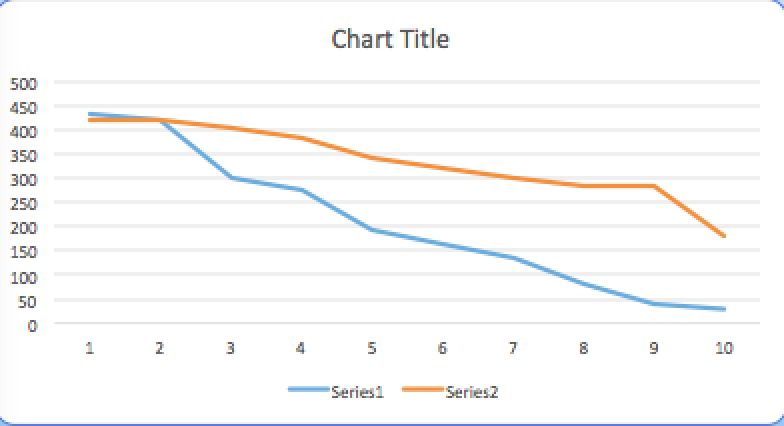
\includegraphics {mopta}


In the robustification of the large data set, we take a conservative approach since our resource of computing is limited. We only consider the case where project i,j fails in the worst scenario, and i is in some set $I \vdash j$. The approach we take is to add other projects in set I that were not previously selected into the plan. Another reason for not deleting failed projects is that the cost for failure does not differ much from project to project, and the deletion will make the remaining projects in the schedule more susceptible to the attack of bad luck. Here we plot how the value in the worst case changes after the robustification for a given budget of W. From the figure we can see that the robust schedule performs much better than the initial schedule in the worst scenario.


%\subsection{Impact of a single bad luck in Scheduling network}
%We begin with the analysis of a simple case, in which only one project is influenced by bad luck. Given the original schedule with a set S of selected projects, T the time of selected projects, and project i is influenced by: 
%\begin{itemize}
%\item Failure.  There're two cases:
%\begin{itemize}
%\item i is in the set of Benefit Jobs. In this case every scheduled projects will start at the scheduled time, since the failure of project i will not have any impact on other projects.
%\item i is in the set of intermediate Projects. A direct consequece is that any project k that requires the successful completion of i, or $M(k,i)==1$ will not be started. Those interemediate projects that were planned to take place after the completion of i and only relevant to the deleted benefit jobs will also be removed from the schedule. The relavance can be determined from the dependency matrix. For the remaining projects in the schedule,  If i is in some set I with $I \succ j$ for a project j, the time of j  and later on projects will be updated. The method for updating the time will be discussed in the Delay part. The algorithm can be summarized as:
%\begin{algorithm}
%\KwData{ Set S of Selected Projects, T Time of Projects, Failed Project i}
%\KwResult{Updated Schedule S', Time T'}
%     S'=S, T'=T\;
%     \ForAll{j in S' with M(j,i)==1}{
%           Remove j from S', Remove $t_j$ from T'\;
%    }
%    \ForAll{ j in S' with M(k,j)==0 for all k in $S'\cap Benefit Projects$}{
%          Remove j from S',Remove $t_j$ from T'\;
%   }
%Update the Time(The detail is similar to the case of delay)\;
%\end{algorithm}
%\end{itemize}
%\item Delay. The analysis here begins with the calculation of updated time. The projects that starts before the scheduled completion time of i will not be affected. An iteration is used to get the updated time for the remainning projects. In each iteration, the project with the earliest scheduled starting time is selected based upon the original scheduled time, the updated completion time of prerequisite projects and ealier conflicting projects. If the completion time for any project j  in the set of Benefit Jobs is beyond the deadline, then the project j is removed together with other intermedate projects that only relevant to j. We could do the computation from beginning again until no projects are removed. The algorithm is as follows:
%\begin{algorithm}
%\KwData{ Set S of Selected Projects, T Start Time of Projects, TF Completion Time of Projects, Delayed Project i}
%\KwResult{Updated Schedule S', Start Time T',Completiong Time TF'}
%    \ForAll{j in S}{
%%           \If($t_j\,\leq\, t_i\,+\,d_i$){
%%            1\;
%%                %Remove j from S, $t_j$ from T\;
%%                %Add j to S', Add $t_j$ to T'\;
%%           }
%%       
%%\Else{
%%               Choose $j\in S$ with the smallest $t_j$ and all previous prerequisites has been satisfied\;
%% $t'_j\,=\,max(t_j, max())$\;
%     \eIf{$t_j\,\leq\, t_i\,+\,d_i$}{
%   go to next section\;
%  Add j to S', Add $t_j$ to T'\;
%   }{
%   Choose $j\in S$ with the smallest $t_j$\;
%  $t'_j\,=\,max(t_j, max(tf_i, i\succ j), max(min(tf_i,i\in I),I\vdash j))$\;
%   Move j from S to S'\;
%   Add $t'_j$ to T';
%   Calculate $tf'_j=t'_j + d_j$ and adds to TF';
%  }
%}
% \ForAll{j in $S'\cap Benefit Projects$}{
%     If{$tf'_j>0$}{
%          Delete j and projects i that only required by j\;
%     }
%}
%Go to the beginning of the Algorithm and repeat the above steps until no projects are deleted.
%\end{algorithm}
%\item Delay and Failure. This will have combined effects upon scheduling network. The analysis follows from the case of Failure and Delay. The approach here is first to consider the impact of failure of projects and then delay. The purpose for this sequence is to remove some projects first, thus reduce the amount of computation.
%\end{itemize}
%
%\subsection{Impact of a budget of bad luck}
%Given a budget of bad luck, we would like to investigate what the worst condition would be like. At this moment there's no way to give the mathematical formulation for the model. A brute force approach is to select all possible choices of bad luck under the current budget, and then compare the updated benefit and select the choice that yields least benefit. However, this method is time consuming and not realistic especially when the size of the network grows very large. A greedy algorithm is developed to estimate the worst case of bad luck. The main idea of the algorithm is to estimate the loss induced by a single event of bad luck taking place on one project, then select the one with highest loss Although the algorithm cannot give theoretical guarantee about the global optimality of the solution.  a it is computationally feasible and provides insight into what the 'weakest' part of the job scheduling network is. The algorithm is as follows:
%\begin{algorithm}
%\KwData{ Set S of Scheduled Projects, T Start Time of Projects, Budget of bad luck W}
%\KwResult{Updated Schedule S', Start Time T'}
%flag=1\;
%\While{flag ==1}{
%  flag=0\;
%  \ForAll{j in S and i in  bad luck with $W_{ji} < W$ and no bad luck happened to j before}{
%      Calculate the Loss of bad luck $L_{ji}$.\;
%  }
% \If{Select the project j with largest ratio $L_{ji}/W_{ji}$}{
%     flag=1\;
%  }.
% Update the schedule and let S=S', T=T'\;
%}
%\end{algorithm}
%
%\section{Exact Mathematical Formulation of the problem}
%In order to construct the exact mathematical formulation, we assume that the whole proecess is 'adaptive', that is, The schedule of time is updated when a delay or failure in projects happens. For example, if in the original schedule there are three chosen projects, project $1 \succ 2$, project $2 \neq 3$, and the sequence is $1-2-3$. Suppose project 1 fails, project 3 can be started immediately and the sequence is $1-3$. Note that it does not imply that the decision maker has knowledge of which project is going to fail or delay, and a project must start if it has been scheduled and all previous requirements are satisfied.\\ 
%
%The following variables are introduced in the optimization model:
%\begin{equation}
%\begin{aligned}
%z_j&\,=\,\mbox{1 if the project j in S is chosen, 0 otherwise}, \forall j \in S\\
%y_j&\,=\,\mbox{1 if the project j in S begins, or incurs or any cost}, \forall j \in S\\
%p_j&\,=\,\mbox{1 if the project j in S is successfully finished and brings about benefit}, \forall j \in S\\
%t_j &\,=\,\mbox{ time the project j starts, if chosen. 0 if j is not chosen},\forall j\in S\\
%\delta_{ij}&\,=\,\mbox{1 if i is ahead of j in time, 0 otherwise}\\
%\alpha_{ij}&\,=\,\mbox{1 if the time of j is after the time of i in the set I }\\
%f_j &\,=\,\mbox{1 if the chosen project j fails. 0 otherwise}\\
%de_j &\,=\,\mbox{1 if the chosen project j delayed but succed. 0 otherwise}\\
%def_j &\,=\,\mbox{1 if the chosen project j delayed and failed}
%\end{aligned}
%\end{equation}
%In the highest level of the optimization problem, we would like to determine which projects to be selected and their scheduled time of start and completion. However, it is usually useless to write down the scheduled time since they are subject to change as a result of bad luck. On the contrary, the order of the projects, once fixed, will not be affected by any failure or delay. Thus we would like to use the order as an alternative to the time while making the decision. Note that since project can be done simultaneously, the only required to indicate the orders is $\delta$.
%The Model contains the following constraints:
%\begin{itemize}
%\item When scheduling the projects:
%\begin{itemize}
%\item for all $i \succ j$:
%\begin{equation}
%z_j \,\leq\, z_i
%\end{equation}
%\item for all $I \vdash j$:
%\begin{equation}
%z_j,\,\leq\,\sum_{i\in I}z_i
%\end{equation}
%\end{itemize}
%\item Consider the delay and failure of the real case
%\begin{itemize}
%\item No more than one kind of bad luck can take place on each project
% 
%\item A project can only be started if it is scheduled. Since we only take a period of time into consideration, an upper bound is added to the starting time and ending time. That is, if a project is started and not finished before the end of the period, it is regarded as failed.
%\begin{equation}
%\begin{aligned}
%&y_j\,\leq\,z_j\\
%&t_j \,\leq\, T_1 y_j\\
%&t_j + d^+_j\,\leq\,T_1\,+\,T_2 (1\,-\,p_j) 
%\end{aligned}
%\end{equation}
%\item A project can only succed if it has started and does not fail because of bad luck:
%\begin{equation}
%p_j\,\leq\,y_j\,(1\,-\,f_j)\,(1\,-\,def_j)
%\end{equation}
%\item For all $i \succ j$, the project j can be started only if project i is successfully completed:
%\begin{equation}
%\begin{aligned}
%&t_j\,+\,M(1\,-\,y_j)\,\geq\, t_i\,+\,d_i\,+\,d_i^+\, de_i\\
%&y_j\,\leq\,p_i
%\end{aligned}
%\end{equation}
%\item For all $i \neq j$, there are several cases. In the first case, neither of the projects, or only one of them  has been started, that is,  the conflict of project i and  project j in time can be neglected. In the second and third case, both projects have been started, either project i needs to be completed ahead of the starting time of project j, or vice versa. $\delta_{ij}\,=\,1$ if $i \succ j$, otherwise its value is 0:
%\begin{equation}
%\begin{aligned}
%&t_j \,+\, M(1\,-\, y_i\,y_j \,+\,1\,-\,\delta_{ij})\,\geq\,t_i\,+\,d_i\,+\,d_i^+\, de_i\,+\,d_i^+\, def_i\\
%&t_i\, +\, M(1\,-\, y_i\,y_j \,+\,\delta_{ij})\,\geq\,t_j\,+\,d_j+\,d_j^+\, de_j\,+\,d_j^+\, def_j
%\end{aligned}
%\end{equation}
%\item For all $I \vdash j$, the neccesary condition for project j to be started is at least one project in the set I has been successfully finished. The auxillary variable $\alpha_i$ is added to indicate which project in the set serve as a prerequisite for the start of j:
%\begin{equation}
%\begin{aligned}
%&y_j\,\leq\,\sum_{i\in I} p_i\\
%&\alpha_{ij}\,\leq\,p_i\\
%&\sum_{i\in I} \alpha_{ij}\,=\,1\\
%&t_j + M(1-y_j)\,\geq\,\sum_{i\in I} \alpha_{ij} (t_i\, +\,d_i\,+\,d_i^+\, de_i)
%\end{aligned}
%\end{equation}
%\end{itemize}
%\end{itemize}
%\begin{equation}
%\begin{aligned}
%\max_{z} \min_{f,de,def}\max_{t} &\qquad \sum_{j\in S, 0\leq t_j/12<3} \gamma^{t_j} \tilde{c}_j\ z_j,+\,\sum_{j\in S, 0\leq t_j/12<3} \gamma^{t_j+d_j} \tilde{b}_j z_j\\
%s.t & t_i\, \leq\, M z_i,\qquad\forall i \in S\\ 
%&\qquad z_j \,\leq\,z_i, \qquad\forall i \succ j\\
%&\qquad t_j\,+\,M(1\,-\,z_j)\,\geq\, t_i\,+\,d_i,\qquad\forall i \succ j \\
%&\qquad t_j + M(1\,-\, z_i\,z_j \,+\,1\,-\,\delta_{ij})\,\geq\,t_i\,+\,d_i\\
%&\qquad t_i + M(1\,-\, z_i\,z_j \,+\,\delta_{ij})\,\geq\,t_j\,+\,d_j\\
%&\qquad 
%\end{aligned}
%\end{equation}
%kkdkal:
%
%\section{Heuristics to solve the problem}
%It is generally very hard to solve problem (\ref{SecondOrProblem}), since both the decision variables for the project manager and the one that brings back luck contain integer variables, and the objective function in the is not convex for both sides of them. Instead of transforming the problem into a single level problem, which turns out almost impossible, an alternative way is to develop some heuristic to find a strategy that has a high tendency to be both robust and productive. One possible choice is to start with the optimal solution in part 1, and add or delete projects to make the schedule more robust to the bad luck.
%
%
%\subsection{Assumption}
%The following assumptions are made for the following analysis:
%\begin{itemize}
%\item For any project which will bring benefits, there will be no other projects that will depend on the project. In other words, all 'intermediate project' has zero benefit. This is typical in real world scenario, since each 'intermediate project' can be regarded as a phase in a large project, and the benefit can be achieved only when the whole chain of projects are successfully finished.
%%\item The schedule of time is updated when a delay or failure in projects happens. For example, if in the original schedule there are three chosen projects, project $1 \succ 2$, project $2 \neq 3$, and the sequence is $1-2-3$. Suppose project 1 fails, project 3 can be started immediately and the sequence is $1-3$. Note that it does not imply that the decision maker has knowledge of which project is going to fail or delay, he or she can only make the 'optimal' change based upon current progress with the assumption that there's no more delay or failure in the future.
%\item Very limited rescheduling is allowed when a delay or failure happens. There're two kinds updates which can be regarded admissable. First, a project can be cancelled if the precedent project fails, or the  delay in previous projects has shown that there is no hope that the final project can be accomplished on time. Second, a project can be delayed if the previous project is delayed. 
%\item Any project cannot take place earlier than scheduled time. For example, if in the original schedule there are three chosen projects, project $1 \succ 2$, project $2 \neq 3$, and the sequence is $1-2-3$. Suppose project 1 fails, project 3 can not be started immediately, it must wait until the original scheduled time. 
%\item If project i and j conflicts in time, the order of the two projects in the updated schedule must remain the same with the original plan if they both successfully started. 
%\item Only selected projects in the original schedule can be chosen when updating the schedule.   
%\end{itemize}
%
%\subsection{Estimation of Worst case in a network of Projects}
%Before taking any measure to add robustness to the schedule, we would like to investigate how bad luck would influence the final total benefits. In fact, it is very difficult to evaluate how the worst situation would be like. We begin with analysis of a simple case, in which there is only a single chain of projects in the original schedule, and the start of second to last project relies upon the successful completion of the previous project. The chain might suffer from the following kinds of bad luck :
%\begin{itemize}
%\item {\sl Failure}. The failure of some project in a single chain will result in the break-up of the whole chain. The later the failure occurs, the more loss there will be, since more intermediate projects means more cost.
%\item {\sl Delay}. The effect of delay is a little complicated. On one hand, an obvious consequence of delay is all the cost and benefits of subsequent projects in the chain are reduced, which appear to be quite trivial since the parameter $\gamma$ is close to 1. However, as there is a deadline for all the projects, delay will probablily lead to the final project's failue of being completed on time. By the assumption that an updated schedule will be made once any bad luck happens, if the delays occurs early enough, the decision maker will gather enough information to ascertain that the final project can only be finished after the deadline. In that case, all the following projects can be cancelled to reduce the loss.
%\item {\sl Delay and Failure} In the case of a single chain, this will have the same effect with failure.
%\end{itemize}
%%For the case with only a single chain of project, it is enough to compare the bad case we can find with the trivial case, in which none of the project is selected and the total benefit is 0. With he 'budget' of bad luck above certain threshold $W_{thres}$, the last project can not be completed successfully, either because the ending time is beyond the time span or some project in the chain fails. A naive estimation for the threshold is given as:
%%\begin{equation}\label{WThres}
%%W_{thres}\,=\,\min (W_{delay}, -log(p_{f,j}), -log((1-p_{f,j})(p_{f,\delta,j})))
%%\end{equation}
%%Where $W_{delay}$ is the minimum amount of bad luck required for the project to be delayed so that it cannot be completed on time. The evaluation of the $W_{delay}$ is a variation of knapsack problem. Which is:
%%\begin{equation}\label{DelayW}
%%\begin{aligned}
%%\min\limits_{z_j} &\qquad -log((1-p_{f,j})(p_{f,\delta,j})) z_j\\
%%&de_j z_j\,\geq\,T_1\,-\,T_{current}+1\\
%%&z_j \in \{0,1\}
%%\end{aligned}
%%\end{equation}
%%Where $T_1$ is the maximum time span, and $T_{current}$ is the current time for the completion of the last project. If there is no solution to the above problem, $W_{delay}$ will be infinity, otherwise it will take the optimal value of the above problem. \\
%
%The naive measure of robustness used here, however,  only shows the risk of failure without taking the potential loss into account. For example, Consider the two chains below(Figure \ref{CompLate}), It is easy to see that they have the same threshold value of bad luck. However, the lower one will suffer more loss when the badluck happens, since more intermediate project have been carried out. 
%
%\subsection{Identification of critical components in the network of schedule}
%Given a schedule. Questions arise as to how to identify the critical component, or intermediate project that is most easilty attacked by bad luck. The effect of failure on network structure is easy to verify, the major difficutlities lies in how the delay influences the completion time of each project. It is generally very hard to do the computation. In the analysis here we would like to borrow the idea of  critical chain 
%\subsection{Robustification of a single chain of project}
%For a single chain of project, $W_{thres}$, though not quite precise, gives an approximation of how robust the current schedule is subject to bad luck. The aim for this part is to increase this naive threshold. The calculation in equation (\ref{WThres}) identifies the weakest part of the chain:
%\begin{itemize}
%\item $W_{thres}\,=\,W_{delay}$. The project is highly vulnerable to delay. The calculation in (\ref{DelayW}) indicates which projects will be delayed in the worst case. One remedy is to replace those intermediate projects that are delayed in the worst case by some other available projects, which might cost more, but has less probability of delay.   
%\item $W_{thres}\,=\, -log(p_{f,j}) or -log((1-p_{f,j})(p_{f,\delta,j}))$. This implies that the structure of the chain is more likely to be destroyed by the failure of some project j. Similar to the case of delay. The approach here is to first verify that whether the 'weakest' project is necessary, or cannot be substituted for the completion of the chain. If it is, then there is nothing we can do about the chain. If it isn't, then we can try to search some project that is 'parallel' to the current project of interest and add the substitute project into the schedule.
%\end{itemize}
%
%\subsection{Evaluation of Robustness of a schedule network}
%Compared with evaluation of robustness of a single chain of network, the estimation of robustness in a schedule network poses a much more challenging problem. The major difficulties mainly lie in the following aspects:
%\begin{itemize}
%\item The identification of impact of each individual project in the network is complicated, or at least computationally expensive. As with the case in the single chain, bad luck might cause a project to fail or delay. In addition, some projects might serve as an intermediate project, or a key step for multiple chains, and the failure of these projects will lead to the failure of completion for those chains.  However, not all consequences are bad for the failure of a project. It is possible that some projects, which were scheduled at some later time because of conflict in time can be started earlier, and some projects which were not included in the original schedule for the same reason can be taken into the plan as long as they could be finished on time and bring benefit. As we have already assumed that if the updated schedule can only contain those projects in the intial schedule, the latter possibility is ruled out. 
%\item In a schedule network, the purpose is to maximize the total benefit of all the chains of projects. In the case of a single chain of projects, if the chain of project fails when the badluck is above some threshold, it is obvious to choose the trivial case. However, in the cae of multiple chains, The failure of some chains is allowed as long as the total benefit is positive, thus the amount of loss in the case of failure should also be taken into consideration.
%\end{itemize} 
%
%
%	\appendix
%%% \section{}
%%% \label{}
%
%%% References
%%%
%%% Following citation commands can be used in the body text:
%%% Usage of \cite is as follows:
%%%   \cite{key}         ==>>  [#]
%%%   \cite[chap. 2]{key} ==>> [#, chap. 2]
%%%
%
%%% References with bibTeX database:
%
%	\section{Reference}
%	\bibliographystyle{elsarticle-num}
%	\bibliography{moptaRefer}
%
%%% Authors are advised to submit their bibtex database files. They are
%%% requested to list a bibtex style file in the manuscript if they do
%%% not want to use elsarticle-num.bst.
%
%%% References without bibTeX database:
%
%% \begin{thebibliography}{00}
%
%%% \bibitem must have the following form:
%%%   \bibitem{key}...
%%%
%
%% \bibitem{}
%
%% \end{thebibliography}

\end{document}



